%\usepackage[T1]{fontenc}
%\usepackage[utf8]{inputenc}

%!TEX ROOT=../diploma-thesis.tex

\chapter{Verifikace a validace}\label{ch:verifikace}

V této kapitole si pop\'{\i}šeme, jak\'y způsobem byla provedena
verifikace naprogramovan\'ych knihoven pomoc\'{\i}
jednotkov\'ych a integračn\'{\i}ch testů~\cite{luo2001software}
a také jak byly knihovny nasazeny při v\'yvoji ukázkového systému.
T\'{\i}m zároveň zvalidujeme koncept frameworku a shrneme v\'yhody
a nev\'yhody jeho použit\'{\i}.

\section{Testován\'{\i} prototypů knihoven}

Prototypy knihoven, jejichž implementaci jsme popsali
v kapitole~\ref{ch:implementace}, byly důkladně
otestovány pomoc\'{\i} sady jednotkov\'ych a integračn\'{\i}ch testů
a t\'{\i}m byla verifikována jejich správná funkcionalita. Způsob
testován\'{\i} knihoven si pop\'{\i}šeme zvlášť pro každou platformu.

V rámci konceptu \textit{continous integration} (\gls{CI})~\cite{fowler2006continuous}
byl kód po celou dobu v\'yvoje verzován systémem Git~\cite{git},
zas\'{\i}lán do centráln\'{\i}ho repozitáře a s pomoc\'{\i}
nástroje Travis \gls{CI}\footnote{https://travis-ci.org/}
bylo automaticky spouštěno jeho sestaven\'{\i} a otestován\'{\i}. Systém
zároveň okamžitě informoval v\'yvojáře o v\'ysledc\'{\i}ch. To
umožnilo v krátkém časovém horizontu identifikovat konkrétn\'{\i} změny
v kódu, které do programu vnesly chybu. T\'{\i}m byla sn\'{\i}žena
pravděpodobnost regrese a dlouhodobě se zv\'yšila celková kvalita kódu.

\subsection{Platforma Java}

Prototyp knihovny pro platformu jazyka Java byl testován pomoc\'{\i}
nástroje JUnit~\cite{junit4}, kter\'y poskytuje veškerou potřebnou funkcionalitu pro
jednotkové i integračn\'{\i} testován\'{\i}. Všechny testy byly spouštěny automaticky
při sestavován\'{\i} knihovny pomoc\'{\i} nástroje Maven~\cite{maven}.

\lstinputlisting[
caption={Př\'{\i}klad jednotkového testu knihovny pro jazyk Java s využit\'{\i}m nástroje JUnit 4},
label={lst:java-testing},
language=Java,
%frame=single,
]
{code/test_example.java}

Ve zdrojovém kódu~\ref{lst:java-testing}
můžeme vidět jednotkov\'y test tř\'{\i}dy \code{BusinessContextWeaver} ověřuj\'{\i}c\'{\i},
že byly správně aplikovány post-conditions daného byznys kontextu, konkrétně
že bylo správně zakryto pole \code{email} objektu \code{user}. Anotace
\code{@Test} metody \code{test()} znač\'{\i},
že metoda obsahuje \textit{test case} a framework JUnit zajist\'{\i}, že bude spuštěna
a vyhodnocena. Statické metody tř\'{\i}dy \code{Assert} ověř\'{\i}, zda uživateli zůstalo
vyplněno jméno, ale emailová adresa ne.

\subsection{Platforma Python}

Prototyp knihovny pro platformu jazyka Python byl testován pomoc\'{\i}
nástroje \code{unittest}~\cite{pythonunittest}, inspirovaného nástrojem
JUnit. Ačkoliv jméno obou nástrojů nasvědčuje, že slouž\'{\i} zejména pro jednotkové testy,
lze je plně využ\'{\i}t i pro integračn\'{\i} testy.

\lstinputlisting[
caption={Př\'{\i}klad jednotkového testu knihovny pro jazyk Python s využit\'{\i}m nástroje Unittest},
label={lst:python-testing},
language=Python,
%frame=single,
]
{code/test_example.py}

Ve zdrojovém kódu~\ref{lst:python-testing} je př\'{\i}klad jednotkového testu tř\'{\i}dy
\code{Identifier} se třemi metodami ověřuj\'{\i}c\'{\i}mi jeho správnou funkcionalitu.
Funkce \code{test\_split()} ověřuje, zda konstruktor správně přij\'{\i}má dva argumenty,
kde prvn\'{\i} z nich je prefix identifikátoru a druh\'y je jméno identifikátoru.
Funkce \code{test\_single()} naopak ověřuje, zda kontruktor správně přij\'{\i}má jeden
argument a rozděl\'{\i} ho na prefix a jméno identifikátoru.
Nakonec funkce \code{test\_str()} ověřuje správnou funkcionalitu převeden\'{\i}
identifikátoru na textov\'y řetězec.

\subsection{Platforma Node.js}

Jelikož tendence ve světě modern\'{\i}ho JavaScriptu je vytvářet knihovny s co nejmenš\'{\i}m polem působnosti,
které jdou kombinovat do větš\'{\i}ho celku, byl prototyp knihovny pro platformu Node.js testován pomoc\'{\i}
kombinace několika nástrojů. Spouštěn\'{\i} testů obstarává knihovna \textit{Mocha}~\cite{mocha}, zat\'{\i}mco
o ověřován\'{\i} a zápis testů ve stylu \textit{Behaviour Driven Development} (\gls{BDD})~\cite{solis2011study}
se stará knihovna \textit{Chai}~\cite{chai}.

\lstinputlisting[
caption={Př\'{\i}klad jednotkového testu knihovny pro platformu Node.js s využit\'{\i}m nástroje Mocha a Chai},
label={lst:nodejs-testing},
language=JavaScript,
%frame=single,
]
{code/test_example.js}

Zdrojov\'y kód~\ref{lst:nodejs-testing} znázorňuje použit\'{\i} knihoven k ověřen\'{\i} správné funkcionality v\'yrazu
\code{IsNotNull}. Konkrétně je nejprve zkonstruován s konstantn\'{\i}m argumentem typu \code{boolean}
s hodnotou \code{true} a je ověřeno, že v\'yraz se vyhodnot\'{\i} jako \code{true}. Následně je zkonstruován
v\'yraz, kterému je předán argument \code{null} a je ověřeno, že v\'yraz se vyhodnot\'{\i} jako \code{false}.

\section{Př\'{\i}padová studie: e-commerce systém}

Abychom mohli navržen\'y a implementovan\'y framework pro centráln\'{\i} správu
a automatickou distribuci byznys pravidel verifikovat v praxi a validovat
jeho myšlenku, bylo nutné vyzkoušet jeho nasazen\'{\i} při v\'yvoji aplikace.
Pro tento účel vznikla v rámci této práce př\'{\i}padová studie na fiktivn\'{\i}m
ukázkovém e-commerce systému využ\'{\i}vaj\'{\i}c\'{\i} architekturu orientovanou na služby.
Na tomto př\'{\i}kladě demonstrujeme schopnost frameworku poradit si s průřezov\'ymi
problémy v rámci \gls{SOA} a také jeho schopnost plnit požadavky identifikované v
sekci~\ref{sec:implementation-requirements}.

\subsection{Use-cases}

Pro ukázkov\'y systém bylo vymodelováno třináct př\'{\i}padů užit\'{\i}
(z anglického \textit{Use case} (\gls{UC})~\cite{bittner2002use}), jejich
přehled je v tabulce~\ref{tbl:use-cases}.

\begin{table}[h]
    \centering
    \begin{tabular*}{\textwidth}{ l l }
        \hline
        \textbf{\#} & \textbf{Use-case} \\
        \hline \hline
        \textbf{UC01} & Nepřihlášen\'y uživatel si může vytvořit zákazn\'{\i}ck\'y účet \\
        \textbf{UC02} & Zákazn\'{\i}k může prohl\'{\i}žet produkty \\
        \textbf{UC03} & Zákazn\'{\i}k může vkládat produkty do koš\'{\i}ku \\
        \textbf{UC04} & Zákazn\'{\i}k může vytvořit objednávku \\
        \textbf{UC05} & Skladn\'{\i}k si může prohl\'{\i}žet produkty \\
        \textbf{UC06} & Skladn\'{\i}k může do systému zadávat nové produkty \\
        \textbf{UC07} & Skladn\'{\i}k může upravovat u produktů stav skladov\'ych zásob \\
        \textbf{UC08} & Skladn\'{\i}k si může zobrazovat objednávky \\
        \textbf{UC09} & Skladn\'{\i}k může upravovat stav objednávek \\
        \textbf{UC10} & Administrátor si může prohl\'{\i}žet objednávky \\
        \textbf{UC11} & Administrátor může upravovat cenu produktů \\
        \textbf{UC12} & Administrátor může vytvářet uživatele (skladn\'{\i}ky) \\
        \textbf{UC13} & Administrátor může mazat uživatele (skladn\'{\i}ky i zákazn\'{\i}ky) \\
        \hline
    \end{tabular*}
    \caption{Přehled use-cases ukázkového e-commerce systému}
    \label{tbl:use-cases}
\end{table}

\subsection{Model systému}

Na obrázku~\ref{fig:example-model} můžeme vidět diagram tř\'{\i}d reprezentuj\'{\i}c\'{\i}ch
kompletn\'{\i} doménov\'y model ukázkového systému.

\begin{itemize}
    \item \textbf{\code{UserRole}} reprezentuje uživatelskou roli v systému.
    \item \textbf{\code{User}} je entita odpov\'{\i}daj\'{\i}c\'{\i} uživateli, ať už zákazn\'{\i}kovi, či zaměstnanci.
    \item \textbf{\code{Product}} popisuje konkrétn\'{\i} produkt v nab\'{\i}dce společnosti a jeho nákupn\'{\i} a prodejn\'{\i} cenu.
    \item \textbf{\code{Order}} odpov\'{\i}dá objednávce, má vazbu na dodac\'{\i} a fakturačn\'{\i} adresu a také na položky objednávky.
    \item \textbf{\code{OrderItem}} reprezentuje položku objednávky a uchovává údaje o počtu objednan\'ych kusů produktu.
    \item \textbf{\code{Address}} je entita popisuj\'{\i}c\'{\i} dodac\'{\i} či fakturačn\'{\i} adresu.
\end{itemize}

\begin{figure}[ht]
    \centering
    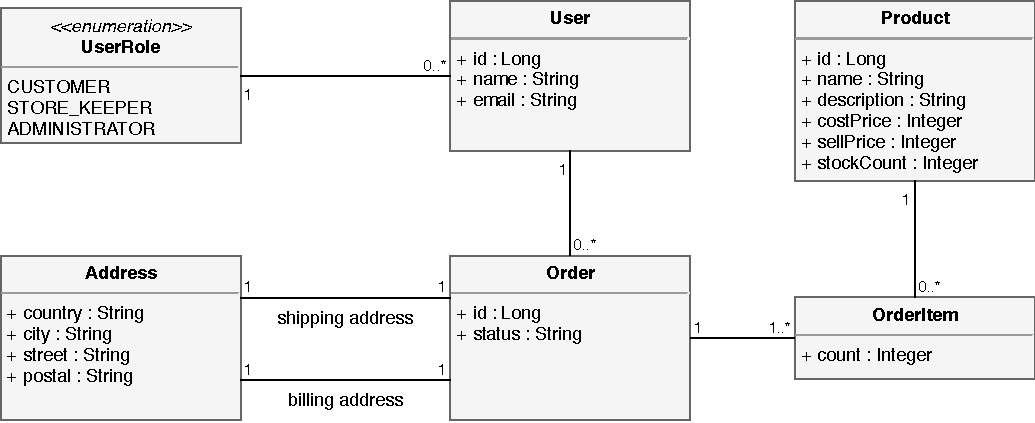
\includegraphics[keepaspectratio=true, width=0.9\linewidth]{figures/example-model.pdf}
    \caption{Diagram tř\'{\i}d modelu ukázkového e-commerce systému}
    \label{fig:example-model}
\end{figure}

Tento model je využ\'{\i}ván v každé ze služeb. Nicméně, ne každá služba využije všechny jeho entity,
ale pouze jejich podmnožinu, kterou potřebuje ke svoj\'{\i} práci.

\subsection{Byznysová pravidla a kontexty}

V tabulce~\ref{tbl:business-rules} je v\'yčet všech dvaceti byznysov\'ych pravidel, která byla
vymodelována pro ukázkovou aplikaci. V tabulce kromě identifikátoru a popisu byznysového pravidla
vid\'{\i}me, na které užitné př\'{\i}pady se pravidlo aplikuje, a jak\'y je typ pravidla
(\textit{pre} pro precondition, \textit{post} pro post-condition).

\begin{table}
    \centering
    \begin{tabular}{ l l c r }
        \hline
        \textbf{\#} & \textbf{Use-cases} & \textbf{Pravidlo} & \textbf{Typ} \\ \hline \hline
        \textbf{BR01} & UC01 & Uživatel nesm\'{\i} b\'yt přihlášen\'y & pre \\ \hline
        \textbf{BR02} & UC02, UC03 & \makecell[c]{Uživatel nesm\'{\i} zobrazovat ani manipulovat \\ s produkty, které nejsou aktivn\'{\i}} & post \\ \hline
        \textbf{BR03} & UC02 až UC04 & \makecell[c]{Uživatel nesm\'{\i} u produktu vidět nákupn\'{\i} cenu, \\ pouze v\'yslednou cenu} & post \\ \hline
        \textbf{BR04} & UC04 & \makecell[c]{Uživatel mus\'{\i} řádně vyplnit doručovac\'{\i} \\ adresu (č.p., ulice, město, PSČ, stát)} & pre \\ \hline
        \textbf{BR05} & UC04 & \makecell[c]{Uživatel mus\'{\i} řádně vyplnit fakturačn\'{\i} \\ adresu (č.p., ulice, město, PSČ, stát)} & pre \\ \hline
        \textbf{BR06} & UC01, UC04 & Zákazn\'{\i}k mus\'{\i} m\'{\i}t vyplněnou emailovou adresu & pre \\ \hline
        \textbf{BR07} & UC04 & Položky objednávky mus\'{\i} m\'{\i}t počet kusů větš\'{\i} než 0 & pre \\ \hline
        \textbf{BR08} & UC04 & \makecell[c]{Položky objednávky mus\'{\i} m\'{\i}t počet kusů menš\'{\i}, \\ než je aktuáln\'{\i} stav skladov\'ych zásob produktu} & pre \\ \hline
        \textbf{BR09} & UC04 & \makecell[c]{Stát mus\'{\i} b\'yt v seznamu zem\'{\i}, \\ do kter\'ych firma doručuje} & pre \\ \hline
        \textbf{BR10} & UC04 & Zákazn\'{\i}k mus\'{\i} b\'yt přihlášen & pre \\ \hline
        \textbf{BR11} & UC05 až UC09 & \makecell[c]{Skladn\'{\i}k mus\'{\i} b\'yt do systému přihlášen \\ a m\'{\i}t roli "Skladn\'{\i}k"} & pre \\ \hline
        \textbf{BR12} & UC05 & \makecell[c]{Skladn\'{\i}k u produktu nesm\'{\i} vidět nákupn\'{\i} cenu, \\ pouze v\'yslednou cenu} & post \\ \hline
        \textbf{BR13} & UC06 & Produkt mus\'{\i} m\'{\i}t jméno s délkou >5 & pre \\ \hline
        \textbf{BR14} & UC07 & Stav zásob produktů mus\'{\i} b\'yt č\'{\i}slo větš\'{\i} nebo rovno 0 & pre \\ \hline
        \textbf{BR15} & UC08 & Skladn\'{\i}k nesm\'{\i} vidět celkov\'y součet cen objednávek & post \\ \hline
        \textbf{BR16} & UC09 & \makecell[c]{Stav objednávky mus\'{\i} b\'yt pouze "přijato", \\ "expedováno" a "doručeno"} & pre \\ \hline
        \textbf{BR17} & UC10 až UC13 & \makecell[c]{Administrátor mus\'{\i} b\'yt do systému přihlášen \\ a m\'{\i}t roli "Administrátor"} & pre \\ \hline
        \textbf{BR18} & UC11 & \makecell[c]{V\'ysledná cena produktu mus\'{\i} b\'yt větš\'{\i} \\ než jeho nákupn\'{\i} cena} & pre \\ \hline
        \textbf{BR19} & UC12 & Skladn\'{\i}k mus\'{\i} m\'{\i}t jméno delš\'{\i} než 2 znaky & pre \\ \hline
        \textbf{BR20} & UC12 & Skladn\'{\i}k mus\'{\i} m\'{\i}t emailovou adresu v platném formátu & pre \\
        \hline
    \end{tabular}
    \caption{Přehled byznysov\'ych pravidel ukázkového e-commerce systému}
    \label{tbl:business-rules}
\end{table}

Dále jsou v tabulce~\ref{tbl:business-contexts} vypsány všechny byznysové kontexty v ukázkové aplikaci.
Některé z nich jsou konkrétn\'{\i} a jsou namapovány na jeden nebo v\'{\i}ce \gls{UC},
jiné jsou abstraktn\'{\i} a slouž\'{\i} ostatn\'{\i} kontexty je rozšiřuj\'{\i}.
Prefixy byly vybrány na základě byznysové domény, ke které se kontext vzahuje, stajně jako
jsou podle domén děleny i jednotlivé služby systému.

\begin{table}
    \centering
    \begin{tabular*}{\textwidth}{ l c l }
        \hline
        \textbf{Identifikátor} & \textbf{Use-cases} & \textbf{Byznysová pravidla} \\ \hline \hline
        \textbf{auth.adminLoggedIn} & - & BR17 \\ \hline
        \textbf{auth.employeeLoggedIn} & - & BR11 \\ \hline
        \textbf{auth.userLoggedIn} & - & BR10 \\ \hline
        \textbf{billing.correctAddress} & - & BR05 \\ \hline
        \textbf{order.addToBasket} & UC03 & BR02, BR08, BR10 \\ \hline
        \textbf{order.changeState} & UC09 & \makecell[l]{BR04, BR05, BR06, BR08, BR09, BR11, \\ BR16} \\ \hline
        \textbf{order.create} & UC04 & \makecell[l]{BR03, BR04, BR05, BR06, BR07, BR08, \\ BR09, BR10, BR16} \\ \hline
        \textbf{order.listAll} & UC08, UC10 & BR11, BR15 \\ \hline
        \textbf{order.valid} & - & BR04, BR05, BR06, BR09, BR16 \\ \hline
        \textbf{product.buyingPrice} & - & BR03 \\ \hline
        \textbf{product.changePrice} & UC11 & BR17, BR18 \\ \hline
        \textbf{product.changeStock} & UC07 & BR08, BR11, BR14 \\ \hline
        \textbf{product.create} & UC06 & BR10, BR11, BR13 \\ \hline
        \textbf{product.hidden} & - & BR02 \\ \hline
        \textbf{product.listAll} & UC02, UC05 & BR02, BR03, BR12 \\ \hline
        \textbf{product.stock} & - & BR08 \\ \hline
        \textbf{shipping.correctAddress} & - & BR04, BR09 \\ \hline
        \textbf{user.createCustomer} & UC01 & BR01, BR06 \\ \hline
        \textbf{user.createEmployee} & UC12 & BR06, BR17, BR19, BR20 \\ \hline
        \textbf{user.delete} & UC13 & BR17, BR21 \\ \hline
        \textbf{user.validEmail} & - & BR06 \\ \hline
        \hline
    \end{tabular*}
    \caption{Přehled byznysov\'ych kontextů ukázkového e-commerce systému}
    \label{tbl:business-contexts}
\end{table}

Na obrázku~\ref{fig:example-system-context-hirearchy} je vizualizována
hirearchie byznysov\'ych kontextů v ukázkovém systému, jejich vazba na \gls{UC}
a také byznysová pravidla, která se v kontextech aplikuj\'{\i}.

\subsection{Služby}

Na obrázku~\ref{fig:example-system} jsou zobrazeny komponenty systému a jejich vzájemné závislosti.
Pro ověřen\'{\i} schopnosti podporovat v\'{\i}ce platforem byly pro implementaci systému využity
jazyky Java, Python a JavaScript v kombinaci s běhov\'ym prostřed\'{\i}m Node.js.
Komunikace služeb prob\'{\i}há pomoc\'{\i} \gls{REST} \gls{API} využ\'{\i}vaj\'{\i}c\'{\i} formát \gls{JSON}.
Specifikace jednotliv\'ych rozhran\'{\i} služeb nen\'{\i} pro tuto kapitolu podstatná a proto se
j\'{\i} nebudeme dále věnovat. Pro demonstrativn\'{\i} účely byly s\'{\i}ťové adresy nastaveny př\'{\i}mo v kódu jednotliv\'ych
služeb. Nicméně, navržen\'y framework nevynucuje tento př\'{\i}stup, a tud\'{\i}ž by složitějš\'{\i}
způsob \textit{service discovery} nebylo problém do systému integrovat.

\begin{figure}
    \centering
    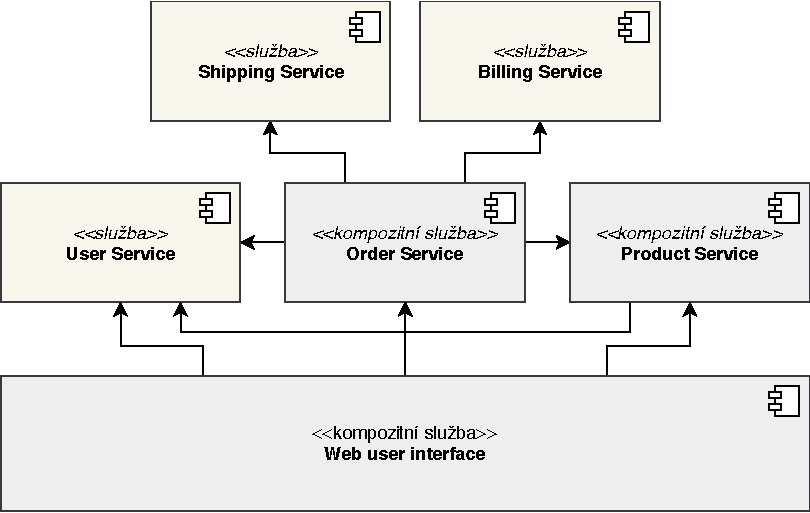
\includegraphics[keepaspectratio=true, width=0.8\linewidth]{figures/example-system.pdf}
    \caption{Diagram komponent ukázkového e-commerce systému}
    \label{fig:example-system}
\end{figure}

\paragraph{Billing service}

Služba \textit{Billing service} má na starosti funkcionalitu t\'ykaj\'{\i}c\'{\i} se fakturace objednávek
a byla implementována v jazyce Java s použit\'{\i}m frameworku Spring Boot~\cite{springboot}.

\paragraph{Order service}

Kompozitn\'{\i} služba \textit{Order service} slouž\'{\i}c\'{\i} pro vytvářen\'{\i} a správu objednávek
byla implementována v jazyce Java a jej\'{\i} \gls{API} bylo sestaveno za použit\'{\i} frameworku Spring
Boot~\cite{springboot}, jak můžeme vidět ve zdrojovém kódu~\ref{lst:order-service-springboot}, kde
je ukázka obsluhy požadavků na v\'ypis zbož\'{\i} v koš\'{\i}ku uživatele.

\lstinputlisting[
caption={Ukázka využit\'{\i} frameworku Spring Boot pro účely Order service},
label={lst:order-service-springboot},
language=Java,
%frame=single,
]
{code/order_service.java}

\paragraph{Product service}

Služba \textit{Product service} realizuje \gls{UC} t\'ykaj\'{\i}c\'{\i} se
prohl\'{\i}žen\'{\i} a administrac\'{\i} nab\'{\i}zen\'ych
produktů a jejich skladov\'ych zásob. Služba byla implementována v jazyce Python.
Pro vytvořen\'{\i} \gls{REST} \gls{API} služby byl využit populárn\'{\i}
light-weight framework \textit{Flask}~\cite{flask}.
Ve zdrojovém kódu~\ref{lst:product-service-flask} můžeme vidět použit\'{\i}
tohoto frameworku pro obsluhu požadavku na v\'ypis všech produktů.

\lstinputlisting[
caption={Ukázka využit\'{\i} frameworku Flask pro účely Product service},
label={lst:product-service-flask},
language=Python,
%frame=single,
]
{code/product_service.py}

\paragraph{Shipping service}

Služba \textit{Shipping service} má na starosti funkcionalitu t\'ykaj\'{\i}c\'{\i} se odes\'{\i}lán\'{\i} objednávek
a byla implementována v jazyce Java s použit\'{\i}m frameworku Spring Boot~\cite{springboot}.

\paragraph{User service}

Služba \textit{User service} realizuj\'{\i}c\'{\i} funkcionalitu t\'ykaj\'{\i}c\'{\i} se uživatelsk\'ych účtů byla
implementována v jazyce JavaScript na platformě Node.js s použit\'{\i}m
frameworku Express~\cite{expressjs}. Ve zdrojovém kódu~\ref{lst:user-service-expressjs}
je ukázka mapován\'{\i} controllerů na jednotlivé metody \gls{URL} \code{/users}.

\lstinputlisting[
caption={Ukázka využit\'{\i} frameworku Express.js pro účely User service},
label={lst:user-service-expressjs},
language=JavaScript,
%frame=single,
]
{code/user_service.js}

\paragraph{Webové uživatelské rozhran\'{\i}}

Služba, která slouž\'{\i} uživatelům ukázkového systému jako webové uživatelské
rozhran\'{\i}, byla implementována v jazyce Java s použit\'{\i}m frameworku Spring Boot~\cite{springboot}.
Na sn\'{\i}mku~\ref{fig:example-screenshot} je vidět UI ukázkového systému,
konkrétně informován\'{\i} uživatele o tom, že se nepodařilo přidat produkt
do koš\'{\i}ku, protože bylo porušeno byznysové pravidlo – koš\'{\i}k nesm\'{\i} obsahovat
v\'{\i}ce než 10 položek.

\paragraph{Centráln\'{\i} správa byznysov\'ych pravidel}

Do ukázkového systému byl nasazen také systém pro centráln\'{\i} správu byznysov\'ych kontextů,
kter\'y je popsan\'y v sekci~\ref{sec:central-administration}. Systém byl napojen na všechny
služby systému, kromě webového \gls{UI}, a bylo úspěšně prokázáno, že lze za běhu systému
dynamicky upravovat byznysové kontexty, resp. jejich byznysová pravidla.

\paragraph{Běhové prostřed\'{\i} služeb}
Pro jednoduché spuštěn\'{\i} celého ukázkového systému byla využita technologie
Docker~\cite{merkel2014docker}, která umožňuje vytvořit virtuáln\'{\i} běhové prostřed\'{\i}
pro aplikaci pomoc\'{\i} kontejnerizace využ\'{\i}vaj\'{\i}c\'{\i} virtualizaci nad operačn\'{\i}m systémem.
Uživatel si nadefinuje tzv. \textit{image}, kter\'y se skládá z jednotliv\'ych vrstev.
Základn\'{\i} vrstvou je operačn\'{\i} systém, dalš\'{\i}mi mohou b\'yt jednotlivé knihovny instalované do systému.
Př\'{\i}klad definice image pomoc\'{\i} technologie Docker můžeme vidět ve zdrojovém
kódu~\ref{lst:docker-image}. Konkrétně se jedná o definici image, kter\'y
rozšiřuje oficiáln\'{\i} image \code{library/node:9.11.1}~\cite{dockernodeimage}
stavěj\'{\i}c\'{\i} nad operačn\'{\i}m systémem \textit{Linux}~\cite{linux},
a přidává vrstvy s prototypem knihovny našeho frameworku pro platformu Node.js.

\lstinputlisting[
caption={Ukázka zápisu Docker image obsahuj\'{\i}c\'{\i} knihovnu pro platformu Node.js},
label={lst:docker-image},
language=Dockerfile,
%frame=single,
]
{code/dockerfile_nodejs.txt}

\paragraph{Spouštěn\'{\i} služeb}
Pro samotné spuštěn\'{\i} byla využita funkce \textit{Compose}, která umožňuje
definovat a spouštět v\'{\i}ce-kontejnerové aplikace. Ve zdrojovém kódu~\ref{lst:docker-compose}
můžeme vidět zápis Order service. Pro jej\'{\i} image je použit \code{filipklimes-diploma/example-order-service}.
V sekci \code{ports} deklarujeme, že služba má m\'{\i}t z vnějšku př\'{\i}stupn\'y port \code{5501}, na kterém poskytuje své
\gls{REST} \gls{API}, a port \code{5551}, nak terém poskytuje své gRPC \gls{API} pro sd\'{\i}lené byzynsov\'ych kontextů. Order service je závislá
na Product, Billing, Shipping a User service, což explicitně specifikujeme v sekci \code{depends\_on},
aby Docker Compose mohl spustit služby ve správném pořad\'{\i}. Nakonec pomoc\'{\i} \code{links} deklarujeme,
že pro kontejner, ve kterém Order Service poběž\'{\i}, maj\'{\i} b\'yt na s\'{\i}ti př\'{\i}stupné služby \code{product}, \code{user},
\code{billing} a \code{shipping}. Vše je popsáno ve formátu \gls{YAML}~\cite{ben2005yaml}, kter\'y je dnes běžně využ\'{\i}ván
pro konfiguračn\'{\i} soubory, kvůli jeho snadné čitelnosti pro člověka a jednoduchému použ\'{\i}ván\'{\i}.

\lstinputlisting[
caption={Ukázka zápisu v\'{\i}ce-kontejnerové aplikace pro Docker Compose},
label={lst:docker-compose},
language=Yaml,
%frame=single,
]
{code/docker_compose.yml}

\section{Srovnán\'{\i} s konvenčn\'{\i}m př\'{\i}stupem}

\goal{Ukázka na konkrétn\'{\i}m př\'{\i}kladě}
Z tabulky~\ref{tbl:business-contexts} vid\'{\i}me, že 60 \% byznysov\'ych pravidel v ukázkovém systému je
využ\'{\i}váno ve v\'{\i}ce kontextech, a polovina je využ\'{\i}vána např\'{\i}č v\'{\i}ce službami.
V tabulce~\ref{tbl:duplication} je přehledně shrnuto, která pravidla jsou využ\'{\i}vána ve kter\'ych službách.
Při použit\'{\i} konvenčn\'{\i}ho př\'{\i}stupu bychom museli tato pravidla implementovat alespoň
jednou pro každou ze služeb, za předpokladu, že by nedocházelo k duplikac\'{\i}m ve službách samotn\'ych.
Manuáln\'{\i} duplikace nav\'{\i}c přináš\'{\i} nutnost synchronizovat podobu pravidla při každém změnovém ř\'{\i}zen\'{\i},
což zvyšuje náklady na v\'yvoj a riziko lidské chyby.

\begin{table}
    \centering
    \begin{tabularx}{\textwidth}{ l X | l X }
        \hline
        \textbf{\#} & \textbf{Použito ve službách} & \textbf{\#} & \textbf{Použito ve službách} \\ \hline \hline
        \textbf{BR01} & user & \textbf{BR11} & auth, order, product \\
        \textbf{BR02} & order, product & \textbf{BR12} & product \\
        \textbf{BR03} & order, product & \textbf{BR13} & product \\
        \textbf{BR04} & order, shipping & \textbf{BR14} & product \\
        \textbf{BR05} & billing, order & \textbf{BR15} & order \\
        \textbf{BR06} & order, user & \textbf{BR16} & order \\
        \textbf{BR07} & order & \textbf{BR17} & (auth), product, user \\
        \textbf{BR08} & order, product & \textbf{BR18} & product \\
        \textbf{BR09} & order, shipping & \textbf{BR19} & user \\
        \textbf{BR10} & (auth), order, product & \textbf{BR20} & user \\
        \hline
    \end{tabularx}
    \caption{Přehled využit\'{\i} byznysov\'ych pravidel ve službách ukázkového systému}
    \label{tbl:duplication}
\end{table}

\goal{V\'yhody našeho frameworku}
D\'{\i}ky použit\'{\i} naš\'{\i} knihovny je však možné každé pravidlo nadefinovat centrálně
a framework se postará o jeho automatickou distribuci do všech m\'{\i}st, kde je potřeba ho aplikovat.
D\'{\i}ky tomu je možno byznysová pravidla, resp. kontexty, spravovat pomoc\'{\i} nástroje pro
centráln\'{\i} správu, kter\'y je součást\'{\i} našeho frameworku. Z toho vypl\'yvá sn\'{\i}žen\'{\i} nároků
na v\'yvoj a sn\'{\i}žené riziko lidské chyby.

\goal{Nev\'yhody použit\'{\i}}
Jako nev\'yhodu použit\'{\i} frameworku můžeme považovat počátečn\'{\i} investici v
podobě integrace knihoven do služeb systému. Zvážit mus\'{\i}me i cenu popisu byznysov\'ych pravidel
v \gls{DSL}, kter\'y se musej\'{\i} v\'yvojáři systému naučit nav\'{\i}c oproti programovac\'{\i}mu jazyku,
ve kterém popisuj\'{\i} služby. Dále je při návrhu systému potřeba identifikovat byznysové kontexty, jejich
hirearchii a vzájemnou vazbu s byznysov\'mi pravidly, aby bylo možno framework efektivně využ\'{\i}vat.
To může vyžadovat v\'{\i}ce času, než klasick\'y návrh.

\goal{Závěr}
Navržen\'y framework tedy oproti konvenčn\'{\i}mu př\'{\i}stupu nab\'{\i}z\'{\i} možnost z\'{\i}skat dlouhodobě
nižš\'{\i} náklady na v\'yvoj za cenu počátečn\'{\i} investice. Architekt softwarového systému mus\'{\i} př\'{\i}padné nasazen\'{\i}
frameworku zvážit z několika úhlů pohledu a posoudit, zda bude životnost systému dostatečně dlouhá a systém
dostatečně velk\'y. Dalš\'{\i}m podstatn\'ym bodem ke zvážen\'{\i} je reálná m\'{\i}ra znovupoužit\'{\i} byznysov\'ych pravidel.
Mohou existovat domény, ve kter\'ych bude nasazen\'{\i} frameworku jistě mnohem vhodnějš\'{\i}, než v jin\'ych.
D\'{\i}ky provedené př\'{\i}padové studii jsme zjistili, že v \gls{SOA} lze efektivně řešit otázku byznysov\'ych pravidel,
potažmo průřezov\'ych problémů obecně, námi navržen\'ym způsobem.

\section{Shrnut\'{\i}}

V této kapitole jsme popsali, jak\'ym způsobem byly testovány prototypy knihoven
pro platformy jazyků Java a Python a pro platformu Node.js. T\'{\i}m jsme verifikovali
jejich správnou fukcionalitu. Dále jsme naspecifikovali a popsali implementaci
ukázkového systému, na kterém jsme provedli př\'{\i}padovou studii použit\'{\i} našeho
frameworku. D\'{\i}ky tomu jsme validovali, že navržen\'y framework je funkčn\'{\i}
a splňuje požadavky identifikované v sekci~\ref{sec:implementation-requirements}.
Nakonec jsme na ukázkovém systému diskutovali srovnán\'{\i} použit\'{\i} našeho frameworku
a konvenčn\'{\i}ho př\'{\i}stupu k návrhu a implementaci softwarov\'ych systému.
